\section{Das Magnetfeld und Teilchen in Feldern}
\subsection{Eigenschaften von Magnetfeldlinien}
\begin{itemize}
	\item \glqq Starten\grqq\ am Nordpol und \glqq enden	\grqq\ am Südpol
	\item Je dichter die Linien, desto stärker ist das Magnetfeld
	\item Magnetfeldlinien haben keinen Anfang und kein Ende, sondern laufen durch den Magnet hindurch
	\item Magnetfeldlinien können durch einen Kompass oder Eisenspäne sichtbar gemacht werden
	\item Die Lorentzkraft wirkt senkrecht zu den Magnetfeldlinien und senkrecht zur Bewegungsrichtung der el. Ladung
	\item Der magnetische Südpol eines Probemagneten richtet sich entlang der Feldlinien zum Nordpol des erzeugten Feldes aus
	\item Magnetfeldlinien berühren sich nie
	\item Änderungen im Magnetfeld breiten sich mit Lichtgeschwindigkeit aus
	\item Feldrichtung ist die, in die eine Kompassnadel zeigen würde
\end{itemize}

\subsection{Magnetfeld von stromdurchflossenen Leitern}
\subsubsection{Magnetfeld eines stromdurchflossenen Leiters}
Der Leiter ist von magnetischen Feldlinien in Form von konzentrischen Kreisen umgeben. \\
\paragraph{Linke-Hand-Regel:} Zeigt der Daumen in Richtung der Elektronenbewegung, so zeigen die Finger der gekrümmten Hand die Richtung des Magnetfeldes an. 
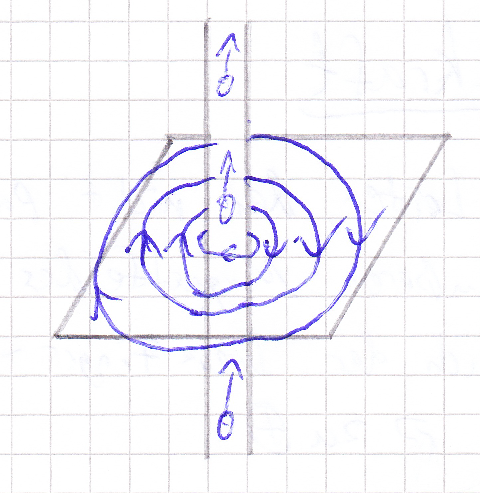
\includegraphics[scale=0.5]{221_magnetfeldlinien}

\subsubsection{Magnetfeld in einer stromdurchflossenen Leiterschleife}
Eine stromdurchflossene Leiterschleife erzeugt ein Magnetfeld wie ein kurzer, dicker Stabmagnet \\
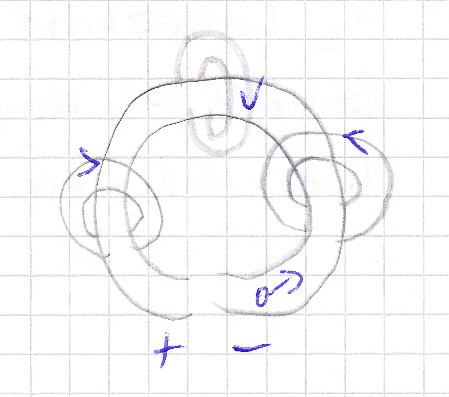
\includegraphics[scale=0.5]{222_magnetfeldlinien}

\subsubsection{Magnetfeld einer langen stromdurchflossenen Spule}
Im inneren ist das Feld homogen, innen laufen die Magnetfeldlinien von Süd nach Nord (wie in jedem Magneten) \\
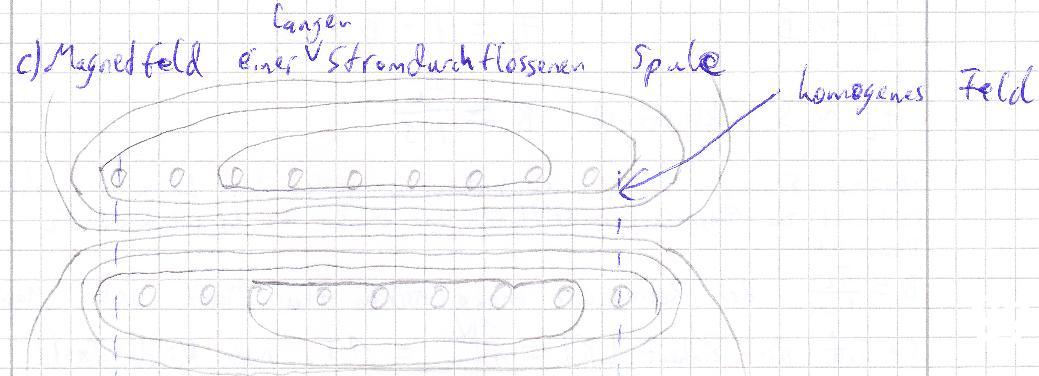
\includegraphics[scale=0.5]{223_magnetfeldlinien}
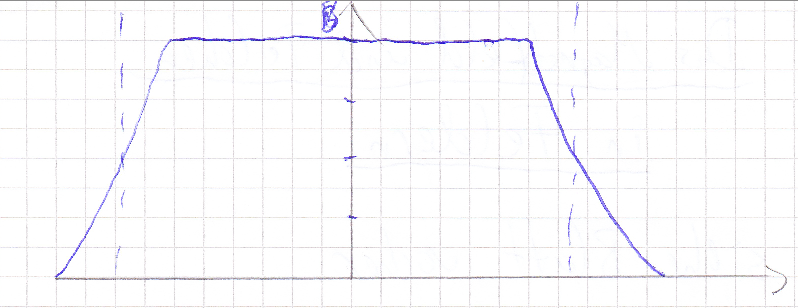
\includegraphics[scale=0.535]{223_homogenitaet}
\newpage

\subsection{Die Lorentzkraft}
Ein stromdurchflossener Leiter, der nicht parallel zu den Feldlinien eines äußeren Magnetfeldes steht, erfährt Lorentzkräfte nach der Drei-Finger-Regel. \\
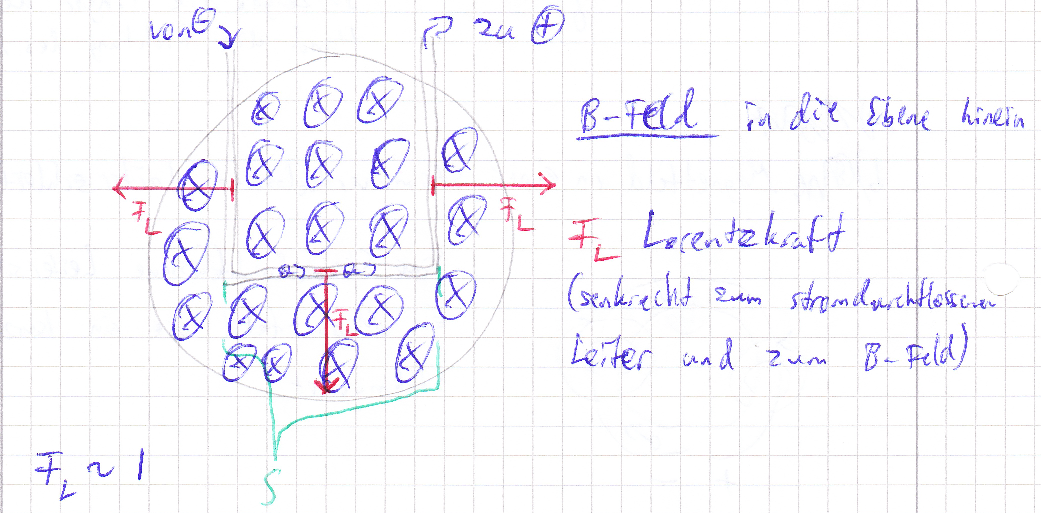
\includegraphics[scale=0.5]{23_Lorentzkraft} \\
$ F_L \sim I $ 
\vspace{1mm} \\
$ F_L \sim B $
\vspace{1mm} \\
$ F_L \sim s $
\vspace{1mm} \\
$ F_L = I \ast B \ast s $
\vspace{1mm} \\
$ B = \frac{F_L}{I \ast s} $

\paragraph{Definition:} Ein vom Strom I durchflossener Leiter der Länge s stehe senkrecht zu magnetischen Feldlinien und erfahre die Lorentzkraft $F_L$. Dann ist $B = \frac{F_L}{I \ast s}$ der Betrag der magnetischen Flussdichte des Magnetfeldes. Sie hat die Einheit $ [B] = \frac{1N}{1A \ast m} = 1T$ nach Nicola Tesla.

\subsection{Magnetische Kraft auf bewegte Ladungen}
Die eigentliche Ursache der Kraft auf einen stromdurchflossenen Leiter ist die Kraft, die im Magnetfeld auf bewegte Ladung wirkt, die sich nicht parallel zum Magnetfeld bewegt. Aus dem Leiterschaukelversuch erhält man:
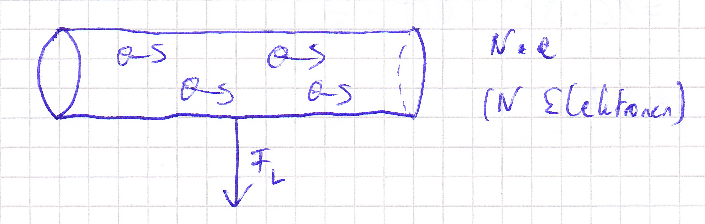
\includegraphics[scale=0.5]{24_leiterschaukel}
\vspace{3mm} \\
$F_L = I \ast B \ast s = \frac{Q}{t} \ast B \ast s = \frac{N \ast e}{t} \ast B \ast s = N \ast e \ast v \ast B$
\vspace{3mm} \\
$ \Rightarrow F_L $ auf ein einzelnes Elektron: $ F_L = e \ast v \ast B $

\newpage

\paragraph{Allgemein gilt:} $F_L = q \ast v \ast B $ \hspace{2mm} wenn \hspace{2mm} $ v \perp B $
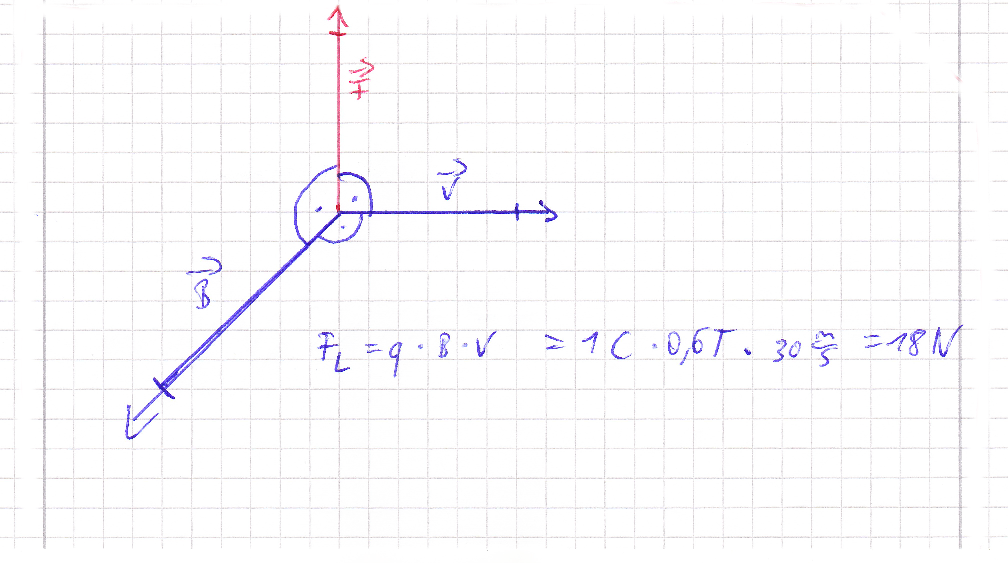
\includegraphics[scale=0.5]{24_lorentzkraft} \\
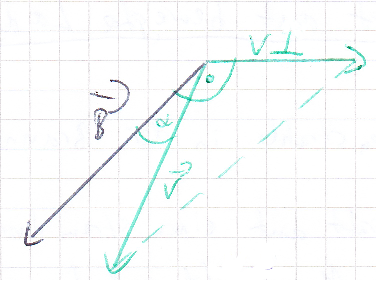
\includegraphics[scale=0.5]{24_lorentzkraft2} \\
$ F_L = q \ast \vec{v} \times \vec{B} $
\vspace{1mm} \\
$= q \ast B \ast \underbrace{v \ast sin(\alpha)} $ \\
\hspace{22.5mm} $ v \perp $

\subsection{Bewegung von Ladungen unter dem Einfluss des B-Feldes}
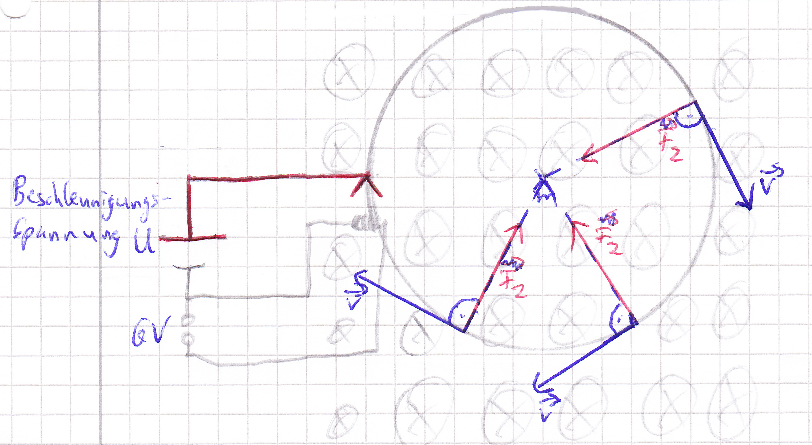
\includegraphics[scale=0.5]{25_zentripetalkraft}

\textbf{Die Lorentzkraft $F_L$ wirkt als Zentripetalkraft $F_Z$}, denn sie wirkt in jedem Punkt senkrecht zur Bewegungsrichtung und ist vom Betrag stets gleich groß. \\
Sie \underline{ändert} also ständig die \underline{Richtung der Bewegung, nicht aber} \\ den \underline{\textbf{Betrag der Geschwindigkeit!}}

\vspace{3mm} 
$ F_L = F_Z$
\vspace{1mm} \\
$ q \ast v \ast B = m \ast \frac{v^2}{r} $
\vspace{1mm} \\
$ q \ast B = m \ast \frac{v}{r} $
\vspace{2mm} \\
$ \frac{q}{m} = \frac{v}{r \ast B} $
\vspace{2mm} \\
$ \frac{e}{m} = \frac{v}{r \ast B} $

\subsubsection{Zusammenfassung: $F_L = F_Z$}
Geladene Teilchen, die mit der Geschwindigkeit $\vec{v}$ in ein homogenes $\vec{B}$-Feld senkrecht zu dessen Feldlinien eintreten, durchlaufen eine Kreisbahn mit dem Radius r. Dieser ergibt sich durch Umformung aus der zentralen Gleichung 
$F_L = F_Z$
\vspace{1mm} \\
$ q \ast v \ast B = m \ast \frac{v^2}{r} $
\vspace{1mm} \\
$ q \ast B = m \ast \frac{v}{r} $
\vspace{1mm} \\
$ r = \frac{m \ast v}{q \ast B} = \frac{v}{\frac{q}{m} \ast B} $
\vspace{5mm} \\
r ist umso größer, je
\begin{itemize}
	\item größer v ist (bei uns: U groß)
	\item kleiner B ist (bei uns: $I_{err}$ klein)
	\item kleiner die spezifische Masse ist
\end{itemize}

\subsection{B- und E-Felder im Verbund}
\subsubsection{Das Massenspektrometer}
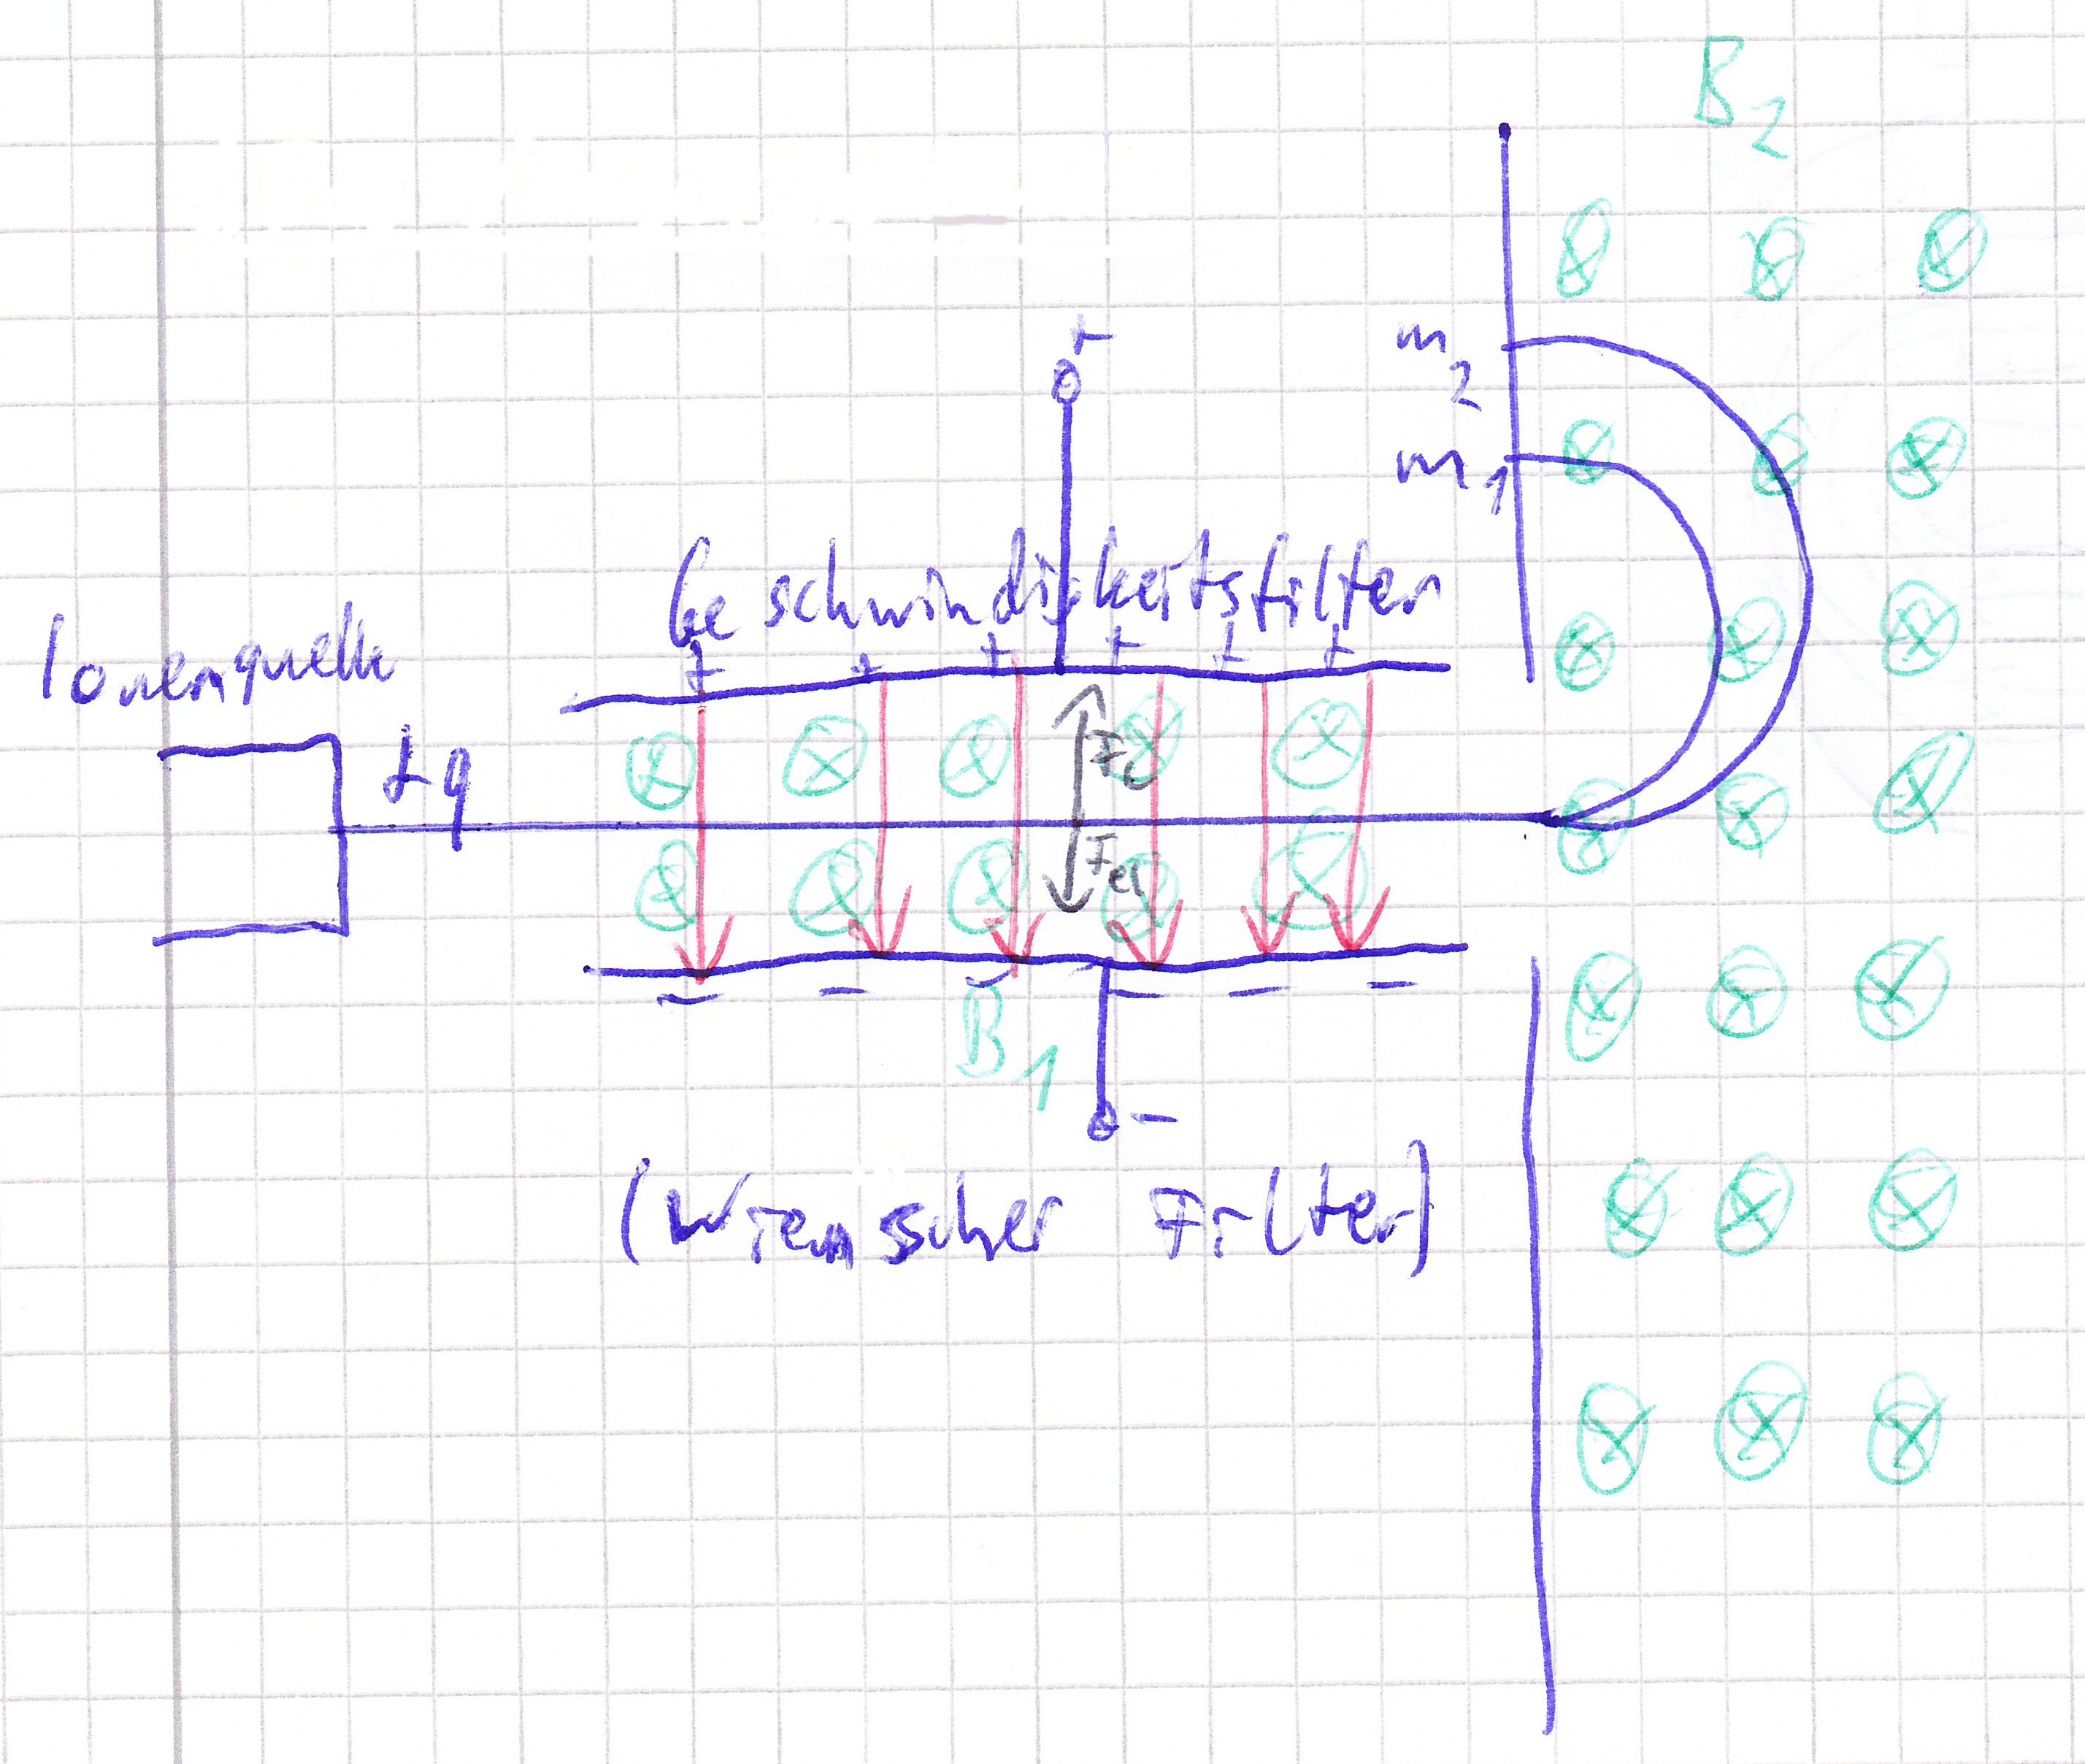
\includegraphics[scale=0.5]{261_massenspektrometer}
\newpage
\paragraph{Funktionsweise eines Wienschen Filters:} Für ein Teilchen, das die passende Geschwindigkeit hat, gilt: 
\vspace{2mm} \\
$ F_L = F_{el} $
\vspace{1mm} \\
$ q\ast v \ast B = q \ast E $
\vspace{1mm} \\
$ v \ast B = E $
\vspace{1mm} \\
$ v = \frac{E}{B} $
\vspace{5mm} \\
$ \Rightarrow $ Zu langsam: Fliegt nach unten
\vspace{1mm} \\
$ \Rightarrow $ Zu schnell: Fliegt nach oben

\paragraph{Funktion des Massenspektrometers:} Aufgrund von $r=\frac{m \ast v}{q \ast B}$ wird r für größere Massen größer ($r \sim m$), wenn alle anderen Größen konstant sind.

\subsubsection{Zyklotron}
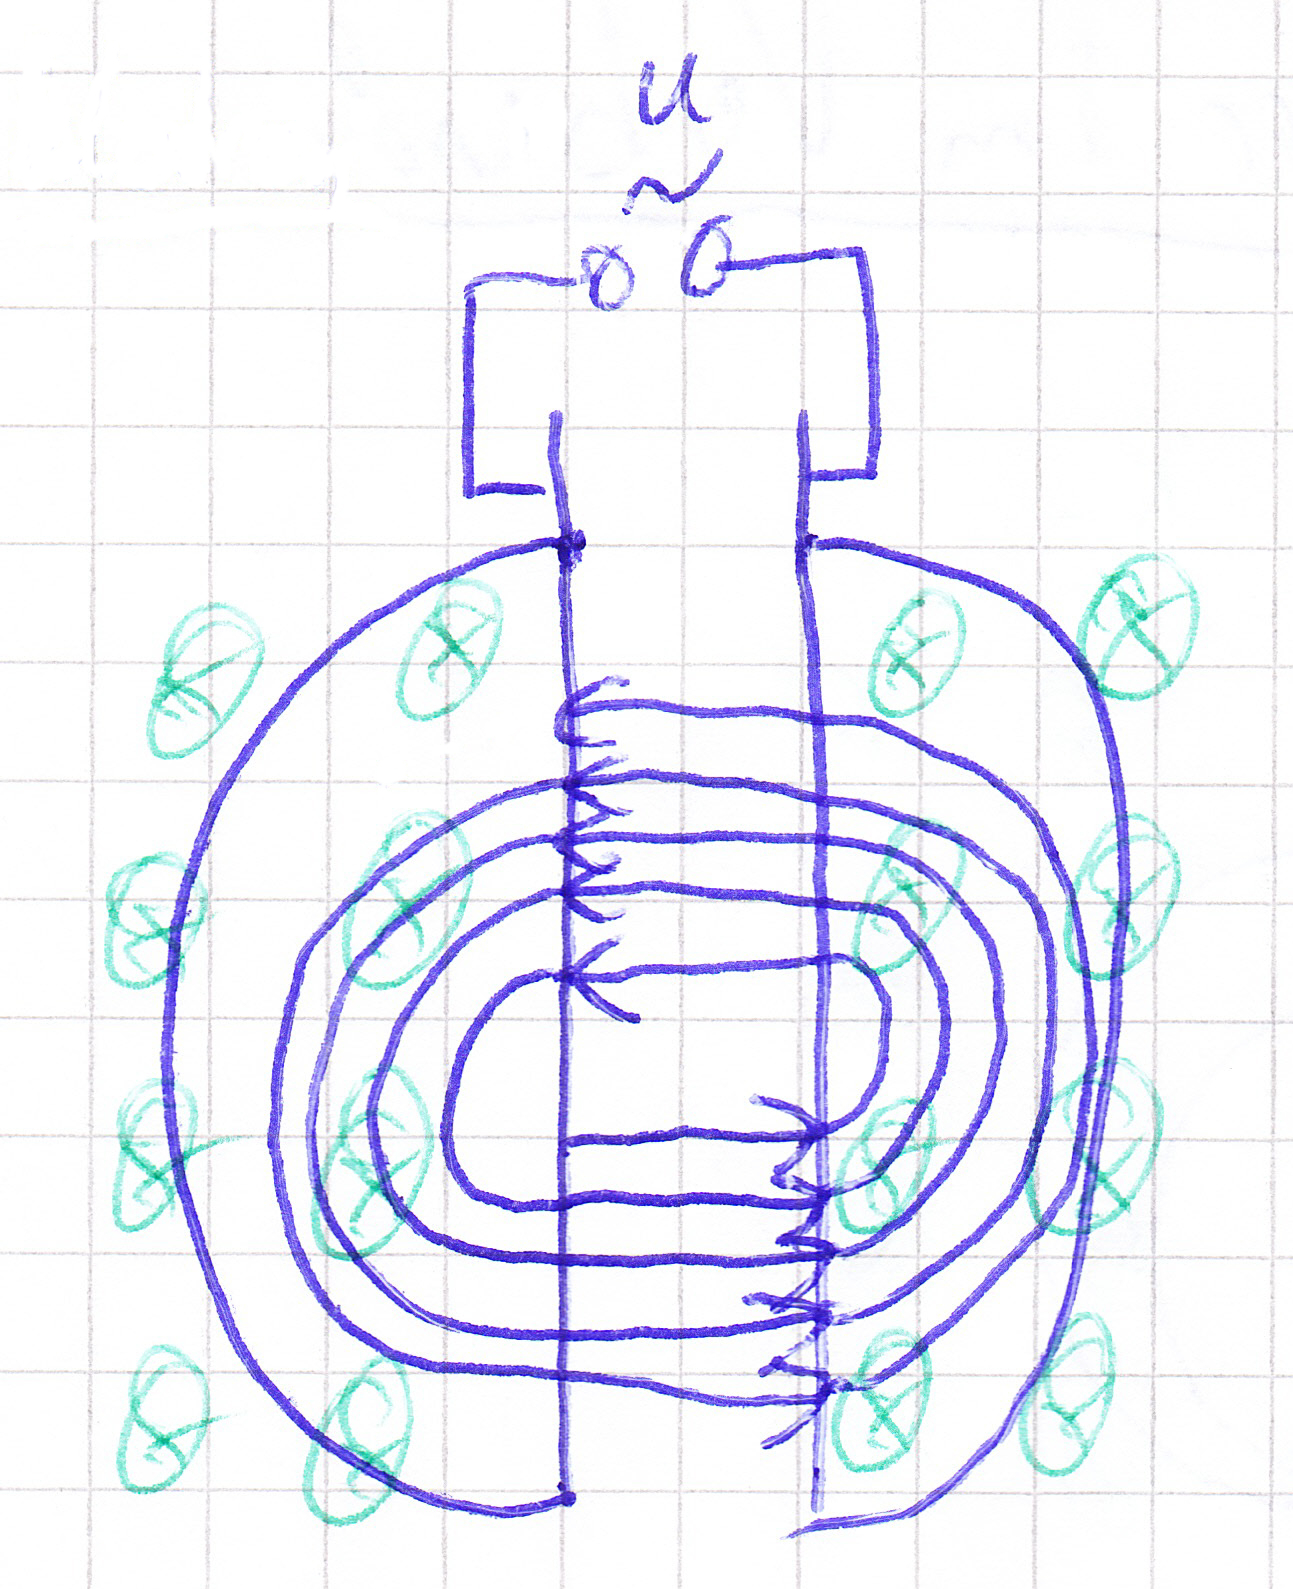
\includegraphics[scale=0.5]{262_zyklotron}

\subsection{Messung von Magnetfeldern}
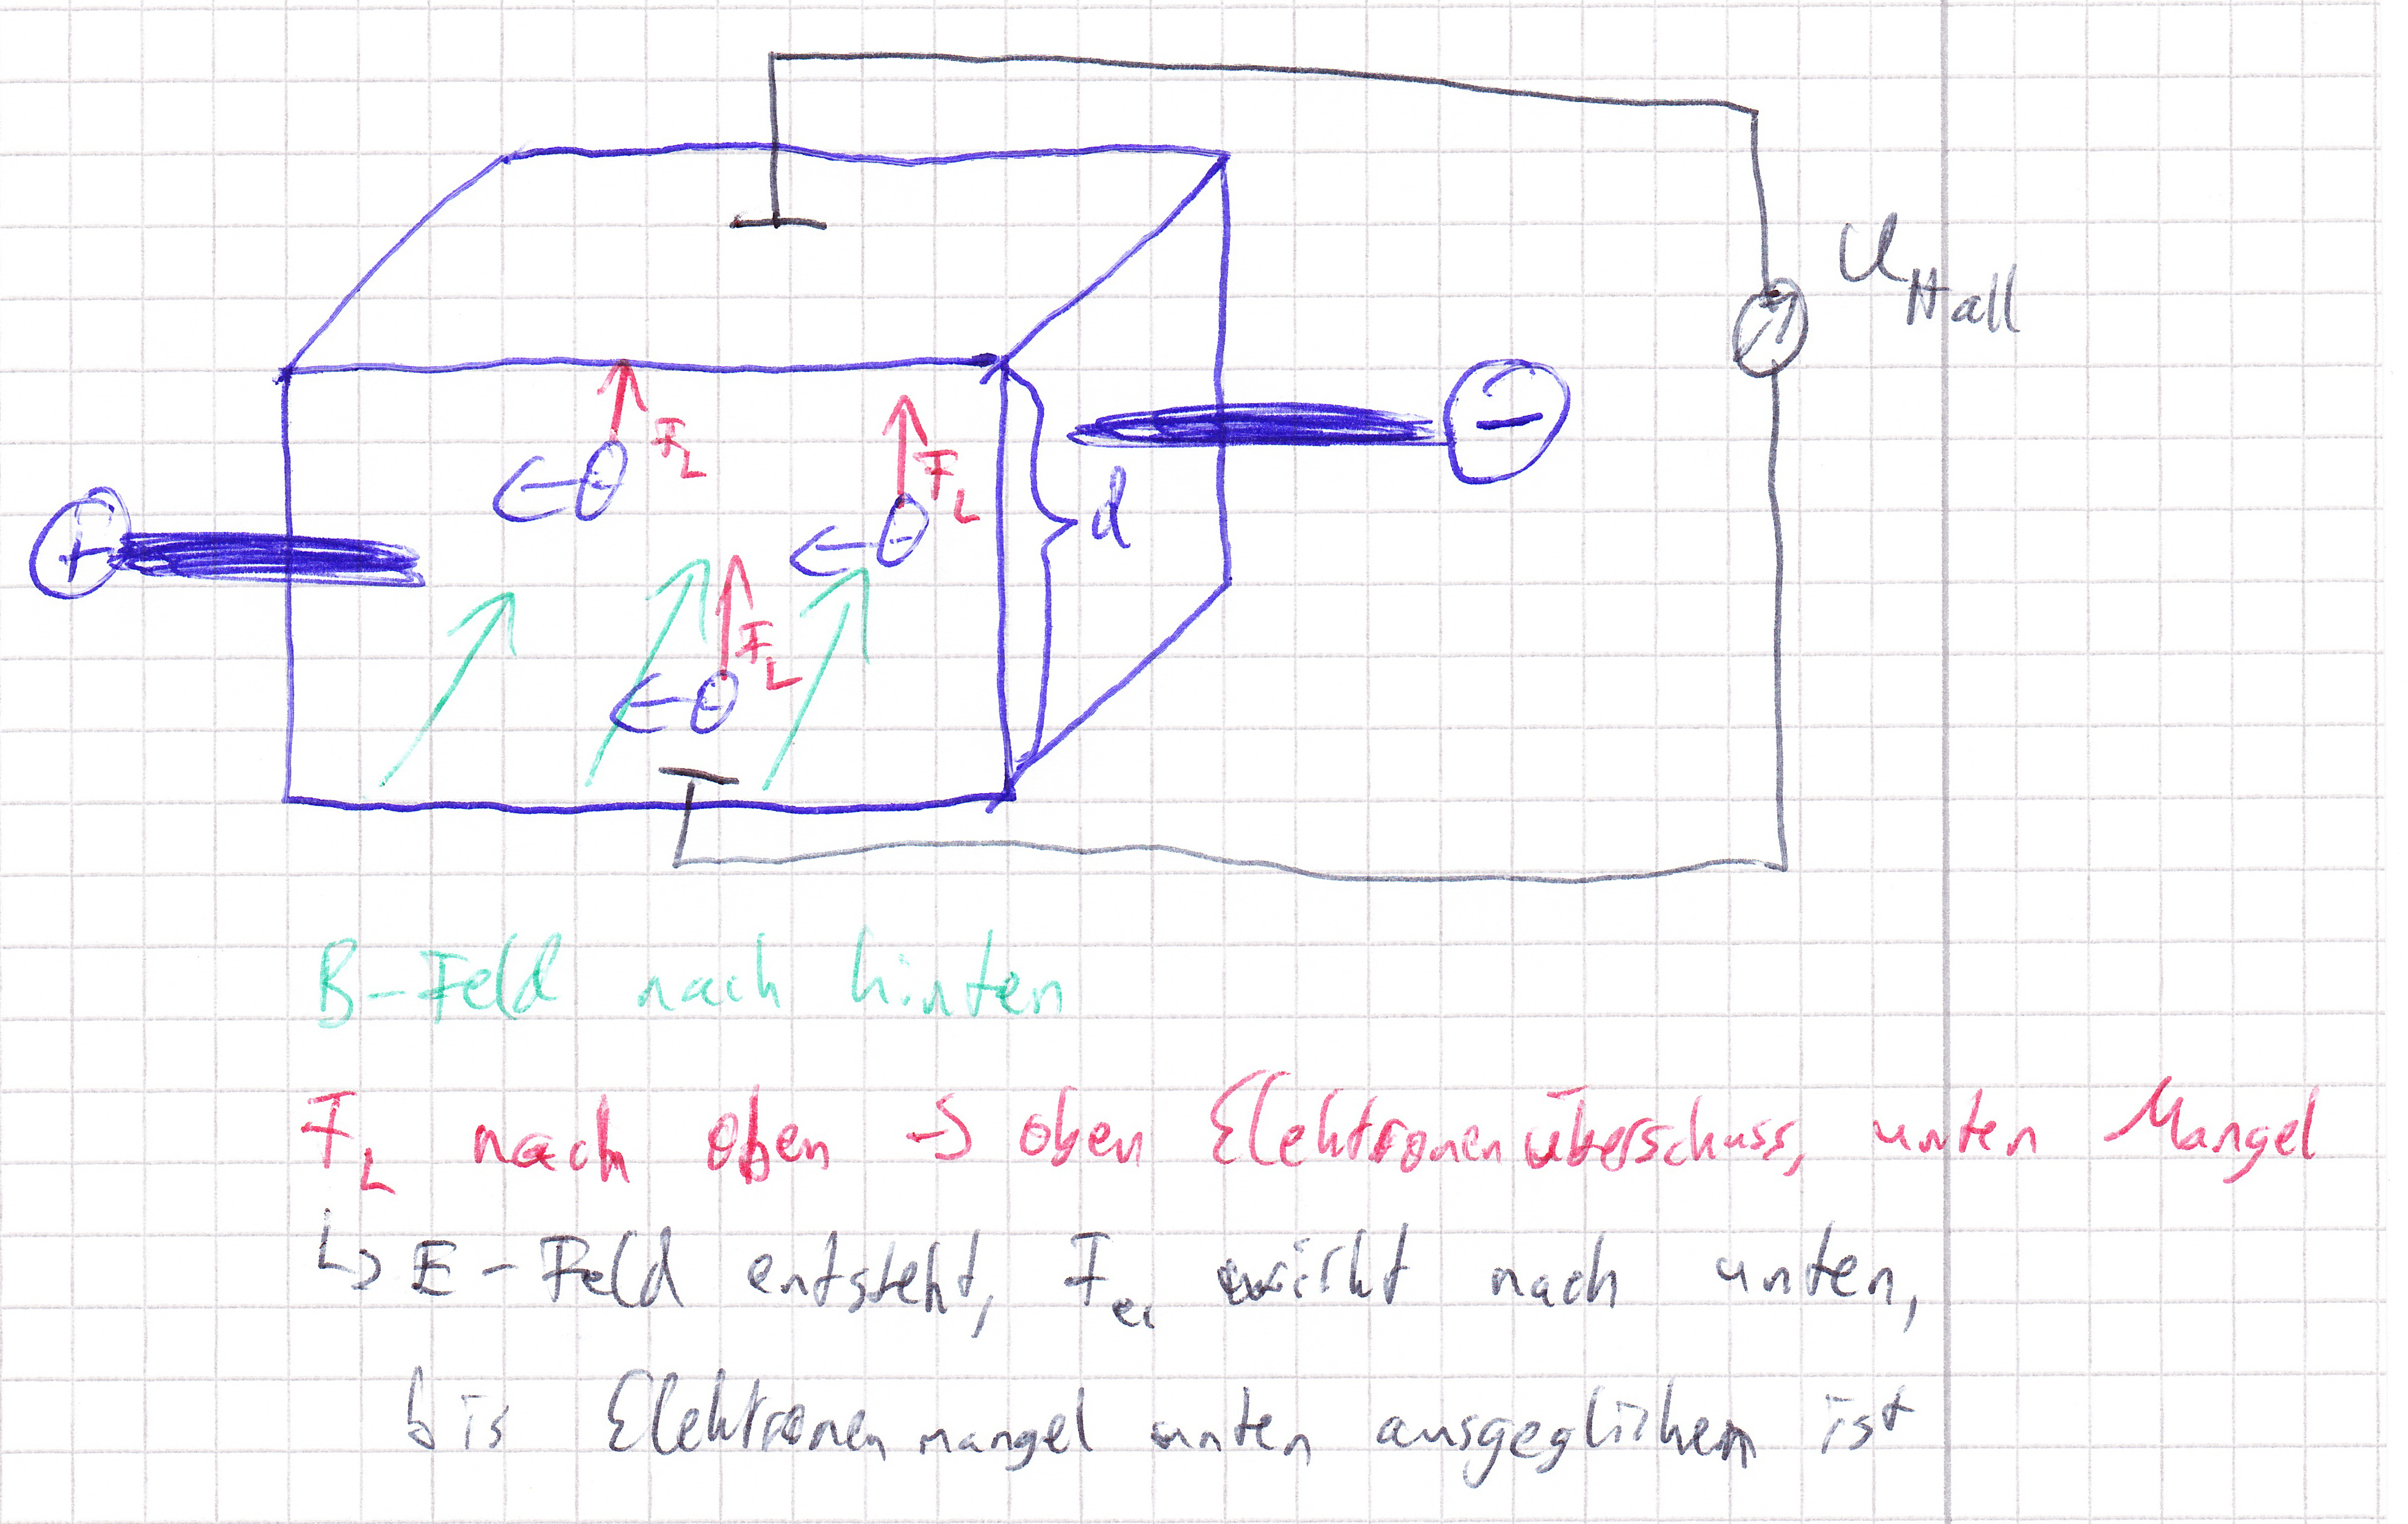
\includegraphics[scale=0.5]{27_hallsensor}\\

\begin{enumerate}
	\item Die Elektronen bewegen sich senkrecht zum B-Feld und werden deshalb nach oben abgelenkt
	\item Durch die Ladungsverschiebung \underline{entsteht} ein E-Feld, das eine $F_{el}$ auf der Elektronen nach unten ausübt.
	\item Die Ladungsverschiebung findet so lange statt, bis $F_L = F_{el}$
\end{enumerate}

Also: 
\vspace{1mm} \\
$F_L = F_{el}$
\vspace{1mm} \\
$ q \ast v \ast B = q \ast E $
\vspace{1mm} \\
$ v \ast B = E $
\vspace{1mm} \\
$ v \ast B = \frac{U}{d} $
\vspace{1mm} \\
$ U_{Hall} = B \ast v \ast d $
\vspace{5mm} 

Hall-Sonden bestehen aus Halbleitern, weil bei ihnen die Anzahl der freien Ladungsträger viel kleiner ist und somit bei gleicher Stromstärke V und damit $U_{Hall}$ größer wird.